\documentclass[preprint]{elsarticle}

\usepackage{amsmath}
\usepackage[linesnumbered,boxed]{algorithm2e}
\usepackage{subfigure}
\usepackage{graphicx}
\usepackage{color}
\usepackage{multirow}

\journal{Information Processing Letters}
\bibliographystyle{elsarticle-num}

\begin{document}
\begin{frontmatter}

\title{A Formal Product Search Model with Ensembled Proximity}


\author{Zepeng Fang}
\author{Chen Lin}
\author{Jian Pei}
\address{Department of Computer Science, Xiamen University, 422 Siming South Road, Xiamen, Fujian, China}

\begin{abstract}
In this paper we study the problem of product search, where products are retrieved and ranked based on how their reviews match the query. Current product search systems suffer from the incapability to measure correspondance between a product feature and its desired property. A proximity language model is presented to embed textual adjacency in the frequency based estimation framework. To tailor for product search problem, we explore strategies for distinguishing product feature and desired property, quantifying pair-wise proximity based conditional probability, and aggregating review opinions at product level. Experiments on real data sets demonstrate good performances of our model. 
\end{abstract}

\begin{keyword}
Information Retrieval\sep Proximity Model\sep Product Search 
\end{keyword}

\end{frontmatter}

%\linenumbers

\section{Introduction}\label{sec:introduction}
Recently, there has been increasing interest in the problem of product search, due to the abundance of online reviews. Revew websites, such as TripAdvisor\footnote{http://www.tripadvisor.com/}, Yelp\footnote{http://www.yelp.com/} and their counterparts in many e-commerce sites, provide listings of products or local businesses on which users are free to comment. Review sites have attracted a huge population of users, and thus have generated an incredible volume of comments. Unfortunately, it is impossible for users to absorb all the information for every candidate product. Product search is then considered to be a prominent tool to explore online reviews and to make smart consumptions.

Product search queries usually consists of consumption preferences on multiple product features. The goal of product search engine is to locate the right products, and rank them based on how they meet the consumption demands. In other words, the general opinions in reviews of the relevant products should be consistent to the desired properties on each product feature respectfully. Such reviews are regarded as supporting evidences. For example, the query in Fig.~\ref{fig:example} seeks for a restaurant with nice decor that serves hot pot. Product B is relevant, since the second review is a supporting evidence which explicitly states that the two features of restaurant satisfy the query need.

\begin{figure}
\centering
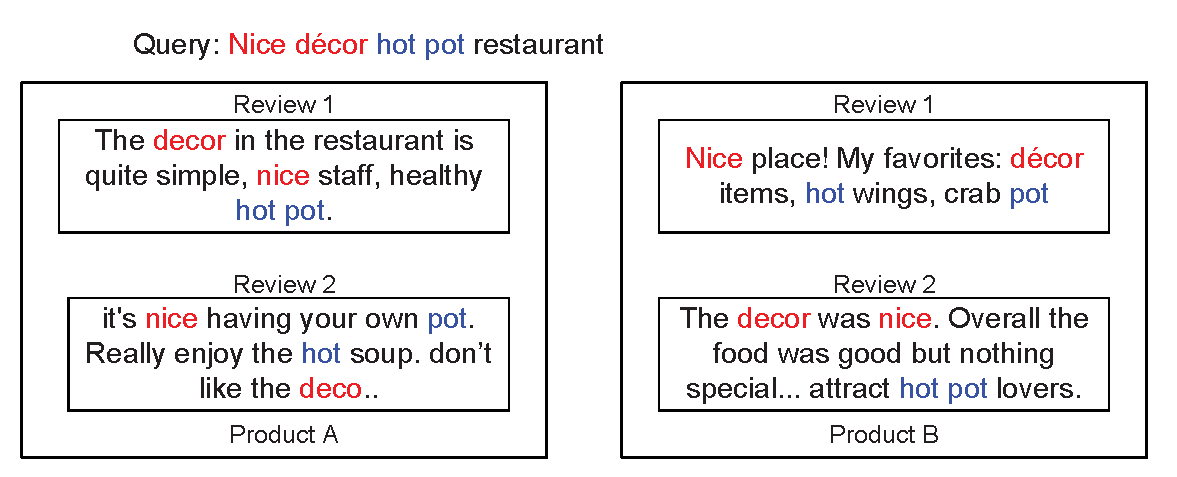
\includegraphics[width=0.5\textwidth]{example.eps}
\caption{An illustration of product search problem}
\label{fig:example}
\end{figure}

To retrieve preferred products from online reviews, several approaches~\cite{Ganesan2012Opinion,Li2011Towards,Duan2013Supporting} have been proposed, most of which are based upon a probabilistic model that measures query-review relevance. They consider a review as supporting, if all the query keywords, including preference keywords and feature keywords, appear in the review. This type of models is limited, as it treats the query as a plain, unstructured ``bag of words'', and does not distinguish the pair-wise correspondence between preferences and features. As illustrated in Fig.~\ref{fig:example}, the first review of product A contains all query keywords. nontheless, it is not a supporting evidence. Because the preferred opinion ``nice'' does not correspond to ``decoration'', instead it is used to describe the feature ``staff''.

The key issue in product search systems is to quantify the relevance between the desired property and the corresponding feature in the reviews. One may easily recognize that relevance is reflected by textual adjacency. In the literature of Information Retrieval, a number of Positional Language Models~\cite{Lv2009Positional,He2011Modeling} have been presented to incorporate term proximity into relevance. Many previous works use traditional IR models to get initial scores of documents and then regularize these scores with a score of proximity between query terms. Positional Language Modles have been shown to significantly enhance the performance of IR systems~\cite{Zhai2008Statistical}. 

However, directly applying PLM for product search is problematic. On one hand, PLM helds a constraint of closeness to all query terms, which might be too strict to harm the accuracy of product ranking. It is possible that a review is a supporting evidence, when many query keywords in the content are remote, as long as the preference keywords are near the corresponding feature keywords. For example, in Fig.~\ref{fig:example}, the average proximity scores for all query terms in review2 for product B is in fact the largest of four reviews. But since both the preferred opinion keywords are close to the feature keywords (``nice '' to ``decor'', ``hot'' to ``pot''), review 2 of product B is the only supporting evidence. Hence it is crucial to segment the query and identify the inner correspondence independently.

On the other hand, given a pair of product feature and preference, PLM is only capable of capturing their association at document level, while product search is implemented at entity level. Each product is linked with a bunch of reviews, where opinions of different reviews may differ, term proximity may vary. The ranking of products is based on the aggregation of supporting evidences. Therefore, it is not trivial to quantify the overall degree of association, given the proximity distributions.

In this paper, we present a formal model to address the above two problems. Following the classic framework of language modeling, we compute the likelihood of observing the query for each product. The query likelihood is factorized to conditional probability of preferred opinion given the product feature. We study the estimation of conditional probability and present three strategies to embed proximity in estimation. Furthermore, we study the effect of aggregated proximity from the review corpus.

\section{Related Work}\label{sec:related}

The great potential of entity search~\cite{Yao2013Unified} has been acknoledged in recent days. Typical entity search paradigms include travel recommendation without a query~\cite{Levi2012Finding}, expert search~\cite{Balog2006Formal}, and query driven product retrieval~\cite{Ganesan2012Opinion,Choi2012CONSENTO,Chen2011Diversifying, Vandic2013Facet, Ganti2010Keyword, Duan2013Supporting}. Product retrieval are either built upon a keyword search framework~\cite{Ganti2010Keyword, Duan2013Supporting}, or a probabilistic language model framework~\cite{Ganesan2012Opinion}. Some of them combine the relevance model with other quality indicators, i.e. best selling prediction ~\cite{Long2012Enhancing}, utility score~\cite{Li2011Towards}, or transition probability from other entries~\cite{Bordino2013Penguins}. Sources for product search are mainly product profiles and online reviews. In retrieving product from reviews, a critical property is reviews are opinionated on different product aspects, and thus demands spetial treatment. In~\cite{Ganesan2012Opinion}, relevance is evaluated by aggregating over all query aspects, and opinion expansion is adopted. To measure relevance of product aspect and opinion, a new indexing unit, Maximal Coherent Semantic Unit is defined and employed in the ranking process~\cite{Choi2012CONSENTO}. The diversify issue is usually addressed in the visualization of search results~\cite{Chen2011Diversifying, Vandic2013Facet}.

Language modeling approaches have been extensively studied in the Information Retrieval community. Various scoring strategies have been proposed in literature, e.g. query likelihood, divergence and relevance and so on~\cite{Zhai2008Statistical}. Beyond general framewoks for computing unigram relevance, one may also want to reward documents in which query terms appear close to each other. To exploit such proximity heuristics, some researchers attempt to capture word dependency by utilizing a larger matching unit, e.g. bigram~\cite{Srikanth2003Incorporating}. To avoid making the indexing space too sparse, Markov Random Field model is presented~\cite{Metzler2005Markov} to collectively scoring unigram, bigram and textual unit within a certain window. Other researchers incorporate query term proximity into an existing retrieval model either directly or indirectly. Directly applying term proximity usually involves defining a combination of relevance score from existing retrieval models and adjusting scores from proximity heuristics~\cite{Buttcher2006Term,Tao2007Exploration}. Indirect methods embed proximity measures and term frequencies in a unified model. In ~\cite{Lv2009Positional}, a language model for each position of a documen that takes into account propogation of word count from other places. Similar strategy is adopted in~\cite{Gerani2010Proximity} for opinion search, seeking blog post that are relevant and opinionated about a user's query. ~\cite{He2011Modeling}extends the well-established BM25 model by taking a linear combination of Ngram proximity based BM25 models for different $N$. This line of researches also include CRTER~\cite{Zhao2014Modeling}, which introduces the concept of cross term -- a pseudo term that is the combination of the individual terms, and is weighted by the intersection of impact propogated from each individual at different positions. Language modeling with proximity enhancements also show great potentials in other tasks, such as machine translation~\cite{Tu2013Exploiting}. 




\section{Model}\label{sec:model}

 Let $D=\{d_1,d_2,\cdots,d_N\}$ be the product universe and $C=\{R_d\}$ is the collection of all reviews, where $R_d$ is the set of review documents for product $d$. The query consists of several preference phrases on multiple product features. We assume the query is segmented, $q=\{(o,f)\}$ in which $o$ denotes the preferred opinion terms and $f$ represents the corresponding feature keywords. Suppose each product is generated from a hidden model $d$, and all the review documents are observations of $d$. Our goal is to estimate the likelihood of generating query from the hidden product model.
\begin{equation}
p(q|d)=\Pi_{(f,o)} p(f,o|d)=\Pi_{(f,o)} p(f|d)p(o|f,d)
\label{equ:likelihood}
\end{equation}

The first part is the probability of selecting feature $f$ from the product, which can be calculated in a frequency based manner. With Dirichlet prior smoothing, we have
\begin{equation}
p(f|d)=\frac{c(f,R_d)+\mu p(f|D)}{|R_d|+\mu}
\label{equ:feature}
\end{equation}

where  $c(f,R_d)$ is the number of times feature keywords $f$ appears in reviews associated with $d$, and $R_d$ is the number of the reviews for $d$, $\mu$ is the smoothing parameter. $p(f|D)$ is the probability of feature $f$ in the product universe $D$ , which can be approximated by average feature frequency over all products.

The second part is the conditional probability of preferred opinion $o$ given feature $f$ in product $d$. It defines the relevance between an opinion $o$ and a feature $f$ in $d$'s reviews. An accurate estimation of $p(o|f,d)$ is an essential step to capture the true correlation of opinion and feature for the candidate product. We will elaborate on this in the next subsection.

\subsection{Conditional Probability Estimation}
%The interpretation of  $p(o|f,d)$ is that, given a query product $d$ and one of its feature $f$, the possibility for any reviewer to choose the opinion $o$ to describe the feature. Intuitively, this quantity will be reflected as term proximity within all reviews. The nearer two terms $f$ and $o$ appear in $R_d$, the more relevant opinion $o$ is to $f$.  Suppose that we have got the term proximity in the product specific reviews, denoted by $d(o,f,R_d)\in \mathbb{R}$, we have three different strategies to integrate $d(o,f,R_d)$.

\textbf{Proximity Parameterized} The first strategy \textbf{PP} is to represent $p(o|f,d)$ as the probability dense function which is parameterized by proximity. Without loss of generality, we assume that given the feature $f$, the author will select opinion $o$ according to a Gaussian distribution $p(o|f,d)\sim N(\mu,\sigma^2)$. Note that the probability for a Gaussian achieves its maximum at its mean, and decreases as the value is distant from the the mean. If the distance between opinion term $o$ and the feature word $f$ is smallest, i.e. $o$ is an adjective that comes before the noun $f$ ,  such as ``nice decor'', then $o$ is most likely to be the opinion to describe the feature. The above observations lead to the functional form

\begin{equation}
p(o|f,d)=\frac{1}{\sqrt{2\pi}\sigma}\exp[(-\frac{d(o,f,R_d)^2}{2\sigma^2})]
\label{equ:parameterized}
\end{equation}

\textbf{Proximity Adjusted} Another strategy \textbf{PA} is to first compute the probability $p(o|f,d)$, then modify it by the proximity. In general, we have $p(o|f,d)=p(o,f|d)/p(f|d)$. From a frequency prospective, the joint probability $p(o,f|d)=\frac{c(o,f,R_d)}{|R_d|}$, the marginal probability $p(f|d)=\frac{c(f,R_d)}{|R_d|}$. Again, to avoid zero probability, we can adopt Jelinek-Merccer smoothing: $p(o|f,d)=(1-\lambda)\frac{c(o,f,R_d)}{c(f,R_d)}+\lambda \frac{c(o,f,C}{c(f,C)}$.

However, the above definition depends only on the co-occurrences, thus ignore the impact of proximity. Intuitively, a larger distance will weaken the credibility of the frequency-based estimation. We employ an exponential weighting scheme to simulate the negative correlation between terms proximity and conditional probability, so that the confidence of a frequency-based estimation $c(o,f,R_d)$ decreases as the absolute distance increases. In order to guarantee the adjusted function is a probability, i.e. $\Sigma_o p(o|f,d)=1$, the dominator $c(f,R_d)$ should be regularized accordingly. Note that, for each observation $f$ in $R_d$, if we ignore the length limit of review, the integration of confidences assigned to all possible $c(o,f,R_d)$ is $\int_{-\infty}^{+\infty}\exp{-x^2}dx=\sqrt{\pi}$. Therefore, to enhance the computational efficiency, the probability is approximated as follows:

\begin{equation}
p(o|f,d)=(1-\lambda)\frac{c(o,f,R_d)\exp{(-{d(o,f,R_d)}^2)}}{c(f,R_d)\sqrt{\pi}}+\lambda \frac{c(o,f,C)}{c(f,C)}
\label{equ:adjusted}
\end{equation}


\textbf{Proximity Censored} Finally we consider probability estimation by directly manipulating the event space. As in the proximity adjusted strategy, $p(o|f,d)$ is proportional to frequency of the event in which the opinion term $o$ and feature keyword $f$ are semantically related. Such a relatedness is invalid, if the two words are far away. Therefore we define the event of observing $o,f$ in a text window of size $\epsilon$. The probability, according to strategy \textbf{PC}, is defined as

\begin{equation}
p(o|f,d)=\frac{c_\epsilon(o,f,R_d)}{ c(f,R_d)}
\label{equ:cencored}
\end{equation}

where  $c_\epsilon(o,f,R_d)=|\{d(o,f,R_d)<\epsilon\}|$, and obviously $\Sigma_o p(o|f,d)=1$


\textbf{Discussion} The presented strategies offer a variety of options to estimate $p(o|f,d)$ with different emphasis. In particular, \textbf{PP} focuses on term proximity, while the rest two combine term frequency and proximity; \textbf{PC} is segmented as it only captures extreme dependency, while the other two is continuous and provide a broader view of semantic correlation; \textbf{PA} takes global frequency over product universe into account, while the remaining two are locally restricted in the current product.

\subsection{Proximity Aggregation}
For a document, the proximity $d(o,f)$ is the absolute difference between the position of $f$ and the position of the nearest observation of $o$, When the product is not associated with a unified profile, we need to study the aggregation of term proximity. Because both terms $f,o$ might appear at multiple positions in the product specific reviews $R_d$. We first present three strategies, based on proximity in a single review.

\textbf{Min} strategy returns the minimal proximity between the opinion and feature in a product. Intuitively, the min strategy suggests that the most significant evidence is adopted, i.e. if only one consumer gives positive feedback, the product will be regarded as relevant.

\textbf{Ave} strategy measures average proximity of two terms in the product reviews. Intuitively, this strategy assumes that all reviews matter, i.e. the product is deemed relevant when the overall feedbacks are good.

\textbf{Max} strategy calculates the maximal proximity between an opinion and its neighboring feature in the product specific reviews. Intuitively, the max strategy only considers the weakest evidence, i.e. the product is relevant if the most critical consumer speaks high of it. 

The above three heuristics are simple and intuitive. The \textbf{Min} strategy and \textbf{Max} strategy are based on single evidence instead of the collective opinions. The \textbf{Ave} strategy is a global measurement, but it is still sensitive to outliers. A typical problem for mining social documents is that usually involves diverse social behaviors. In the setting of product search, reviews for a spcific produc generally contain quite distinct, or even opposite opinions. The uncertainty of language usage and credibility of each user are also factors that contribute to the diversity of product reviews. As a result, we may need a more accurate measurment to reflect the collected opinions on the required product features. For that reasoning, we present a \textbf{ClusterMin} strategy as follows. 

First we represent each review $r \in R_d$ as multiple $V-$dim vectors $r^o$, each for a product feature in the query $o \in q$. The $v-$th element of the feature specific review vector is the minimal distance $r^o_v = \min_{v\in r} d(o,v)$ between the given product feature $o$ and the $v-$th word of the opinion lexicon in the review. We adopt a K-means algorithm to cluster all reviews $r\in R_d$ for product $d$. The centroid of each cluster is also represented by multiple feature specific vectors. In the assigning step, calculate the distance between a review and a centroid $s^k$in cluster $k$ by the combination of feature specific Euclidean distance $\|r-s^k\|_2=\Sigma_o\|r^o-s^{o,k}\|_2$. As opininons are naturally devided into three categories: positive, neutral and negative, we set $K=3$ for clustering.  When the clustering converges, we choose the cluster centroid which has the nearest query specific feature-opinion distance $s^i=s^k|\min_{k=1 \rightarrow 3} \Sigma_{<o,f> \in q}s^{o,k}_f$, and set the aggregated distance as the corresponding element defined by the cluster centroid $d(o,f)=s^{o,i}_f$.


\section{Experiment}\label{sec:experiment}

We evaluate our model with the open benchmark~\cite{Ganesan2012Opinion}. The data set consists of reviews for hotels in different cities and cars of various modules. The queries are natural language formatted. For the purpose of this study, only queries which contain both opinions and associated product features are remained. Ground truth is manually annotated by the authors~\cite{Ganesan2012Opinion}. Statistics of experimental data set is show as Tab.~\ref{tab:data}.


\begin{table}
\small
	\centering
		\begin{tabular}{|c|c|c|c|}
		\hline
		\multicolumn{2}{|c|}{Hotels}& \multicolumn{2}{|c|}{Cars}\\\hline
			No. Cities	& 5 & No. Modules & 3 \\\hline
			Avg. No. Hotels	& 143.2 & Avg. No. Cars & 199.3 \\\hline 
			Avg. No. reviews per hotel & 60 & Avg. No. reviews per car & 67.7 \\\hline
			Avg. document length & 1219.4 & Avg. document length & 1097.3 \\\hline
			Avg. No. Queries & 5 & Avg. No. Queries & 5 \\\hline
		\end{tabular}
		\caption{Statistics of Data Sets}\label{tab:data}
\end{table}


The proposed retrieval model is implemented on the Terrier\cite{Ounis2006Terrier} platform. The index structure is modified to record the position of each term appearence. To enhance efficiency, reviews for a single product are merged to a unified document unit. Term distance across reviews is assigned a large value $400$. In preprocessing, stop words are not removed, porter stemmer is adopted.

\subsection{Performance of Query Segmentation}\label{sec:exp-query}
We segment queries based on the occurences of features and/or opinions. Each product feature is paired with the most adjacent opinion in the query. The product features and opinions are learnt from the corpus by first discovering association rules, then use the value of frequency to prune the nouns in most frequent rules as features. As a pre-processing step, we also compare the performance of query segmentation with two other strategies, including: (1) LSR~\cite{Hu2006Opinion}: product feature extraction by class sequential rules in the corpus; (2)DP~\cite{Qiu2011Opinion}: co-extraction of opinions and features by double propagation in the corpus. We use three common measurements, namely recall, precision and F-score.

\begin{table}
\center
\begin{tabular}{|c|c|c|c|}
\hline
Metric & LSR &	DP &	Ours \\\hline
recall &	0.9062 	& \textbf{1.0000} & 0.9813\\\hline
precision	& 0.0039 &	0.3043 & \textbf{1.0000} \\\hline
f-score	& 0.0076	& 0.3050 & \textbf{0.308}  \\\hline
\end{tabular}
\caption{Comparative performance of query segmentation}\label{tab:queryseg}
\end{table}
As illustrated in Tab~\ref{tab:queryseg}, all three strategies obtain high recall rates. However, LSR performs poorly in term of precision, leading to a very bad result in term of f-score. Our frequen. Our method is better than DP in terms of precision and f-score, but it is slightly worse than DB in term of recall. The possible reason is that DB make use of the result of opinion classification, thus may introduce noise in product feature identification. In query segmentation, A precise segmentation is important to proximity language models, because otherwise the proximity constraints are inaccurate. In the next subsections, we adopt the association rule based method to partition queries.

\subsection{Conditional Proabability Strategy}
We adopt NDCG as the evaluation metric for ranking experiments. Normalized discounted cumulative gain (NDCG) measures the accuracy of a ranking system, in which the score for result at the $k$-th position is computed as $DCG_k=\Sigma_{i=1}^{k}\frac{s_i-1}{\log (i+1)}$, where $s_i$ is the associated score for each product in the ground truth. We report normalized $DCG_{10}$ for the top 10 results, compared with the ideal ranking list. 

We first tune the smoothing parameter $\mu$ for each strategy. The aggregation stragegy is \textbf{Min}. As shown in Fig.\ref{fig:muPP},\ref{fig:muPA},\ref{fig:muPC}, the smoothing parameter $\mu$ for good performance tends to be large. A larger $\mu$ indicates that the feature probability relies more on the global feature probability $p(f|D)$. It is reasonable since a product is associated with a limited number of features, and the reviews usually inclines to cover all these features. Thus the global probability of sampling a feature is a more stable estimate. Also, we observe that with the effect of decaying confidence in the \textbf{PA} significantly shrinks the smoothing parameter $\mu$.

Next we report the effect of strategy specific parameters in Fig.~\ref{fig:sigmaPP},\ref{fig:lambdaPA},\ref{fig:epsilonPC}. We need to point out that \textbf{PP} and \textbf{PA} are not very sensitive to parameters, as the worst results still outperforman comparative baselines in Tab.~\ref{tab:comparative}. Best performance for \textbf{PP} is achieved when $\sigma^2$ is around $200/3$. For a Gaussian distribution with zero mean, $99.7\%$ of the data points are in the range of $[-3\sigma^2,+3\sigma^2]$, which is in line with our assumption that each product feature should at least appear in the same passage with the corresponding opinion (passage length =400 as mentioned above). Best performance for \textbf{PA} is oabtained by $\lambda<0.5$, which suggests the confidence plays a more significant effect than the global statistic. However $\lambda$ is close to $0.5$, the effects are balanced out over the corpus. \textbf{PA} strategy is sensitive to the window size.$\epsilon=1$ performs best, which means when an opinion is directly adjacent to it associating feature, it is the most relevant. In general, the proximity constraints are higher for product search problem, especially for corresponding feature-opinion pairs, compared with other entity search tasks.  

\begin{figure}
\subfigure[NDCG$@$10 for various $\mu$, with $\sigma=200/3$]{
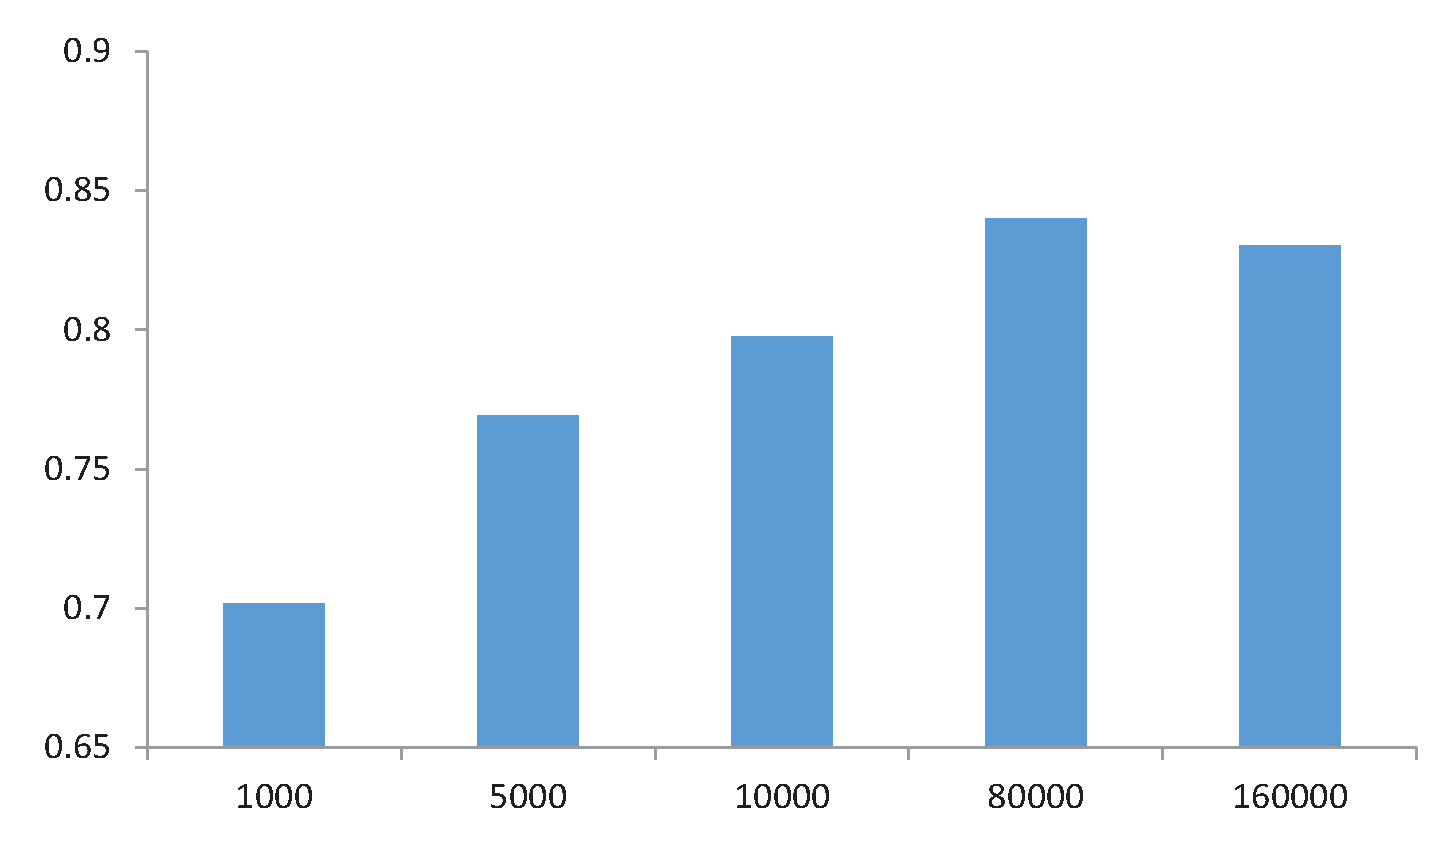
\includegraphics[width=0.5\textwidth]{muPP.eps}
\label{fig:muPP}
}
\subfigure[NDCG$@$10 for various $\sigma$, with $\mu=80000$]{
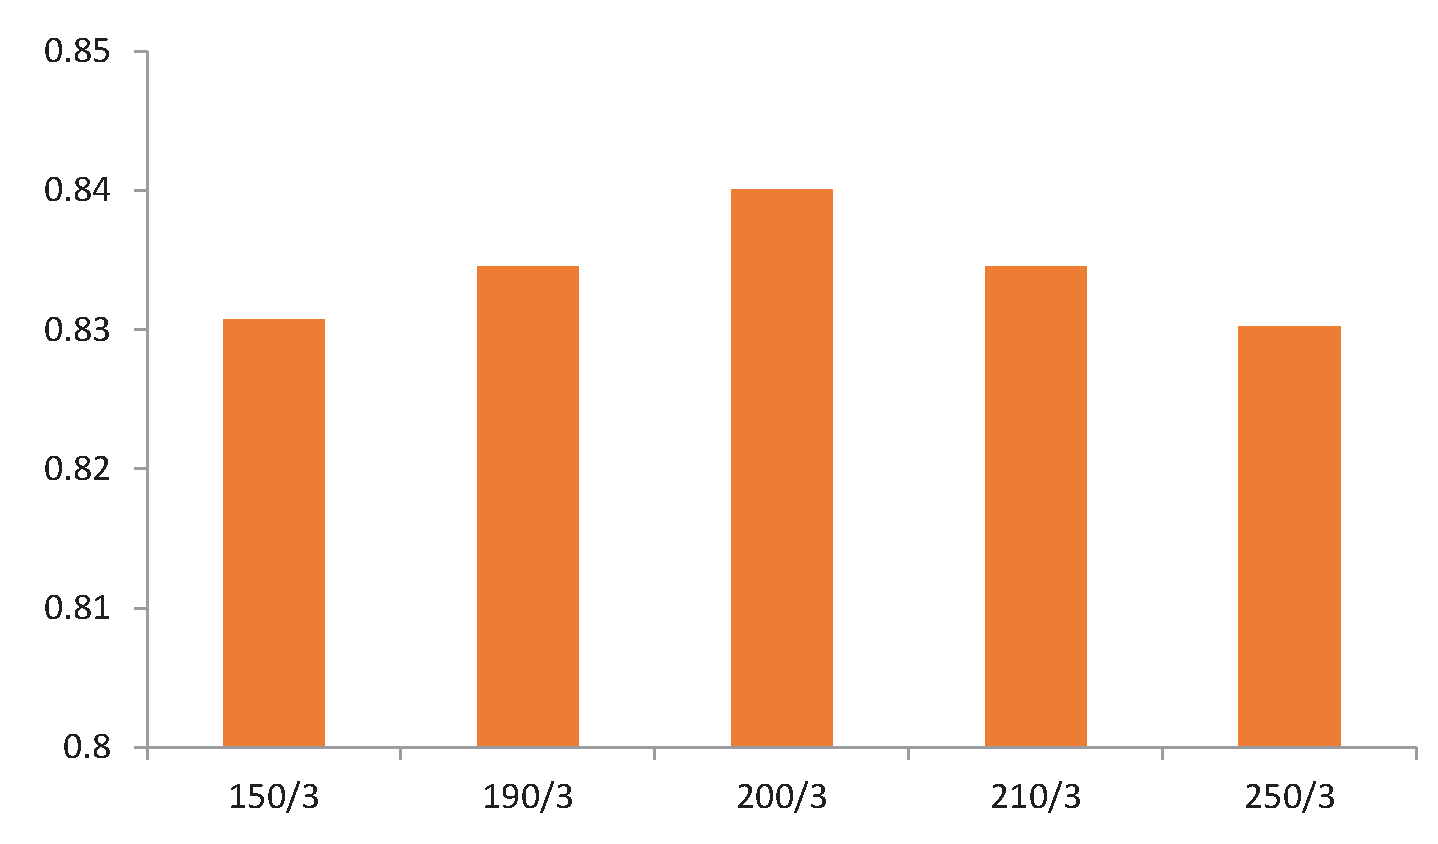
\includegraphics[width=0.5\textwidth]{sigmaPP.eps}
\label{fig:sigmaPP}
}
\caption{Parameter tuning for \textbf{PP} strategy}\label{fig:PP}
\end{figure}


\begin{figure}
\subfigure[NDCG$@$10 for various $\mu$,with $\lambda=0.2$]{
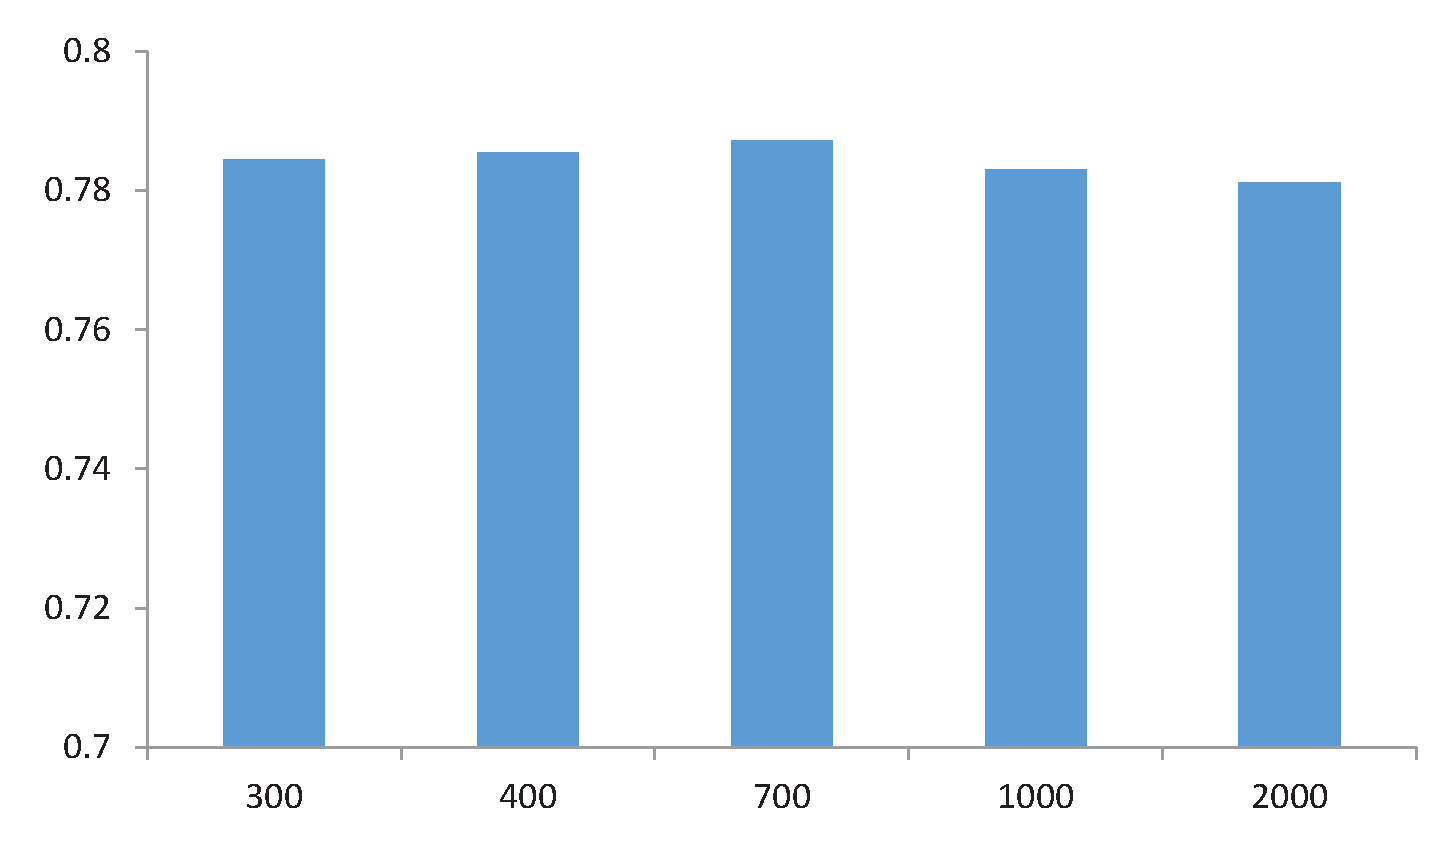
\includegraphics[width=0.5\textwidth]{muPA.eps}
\label{fig:muPA}
}
\subfigure[NDCG$@$10 for various $\lambda$,with $\mu=700$]{
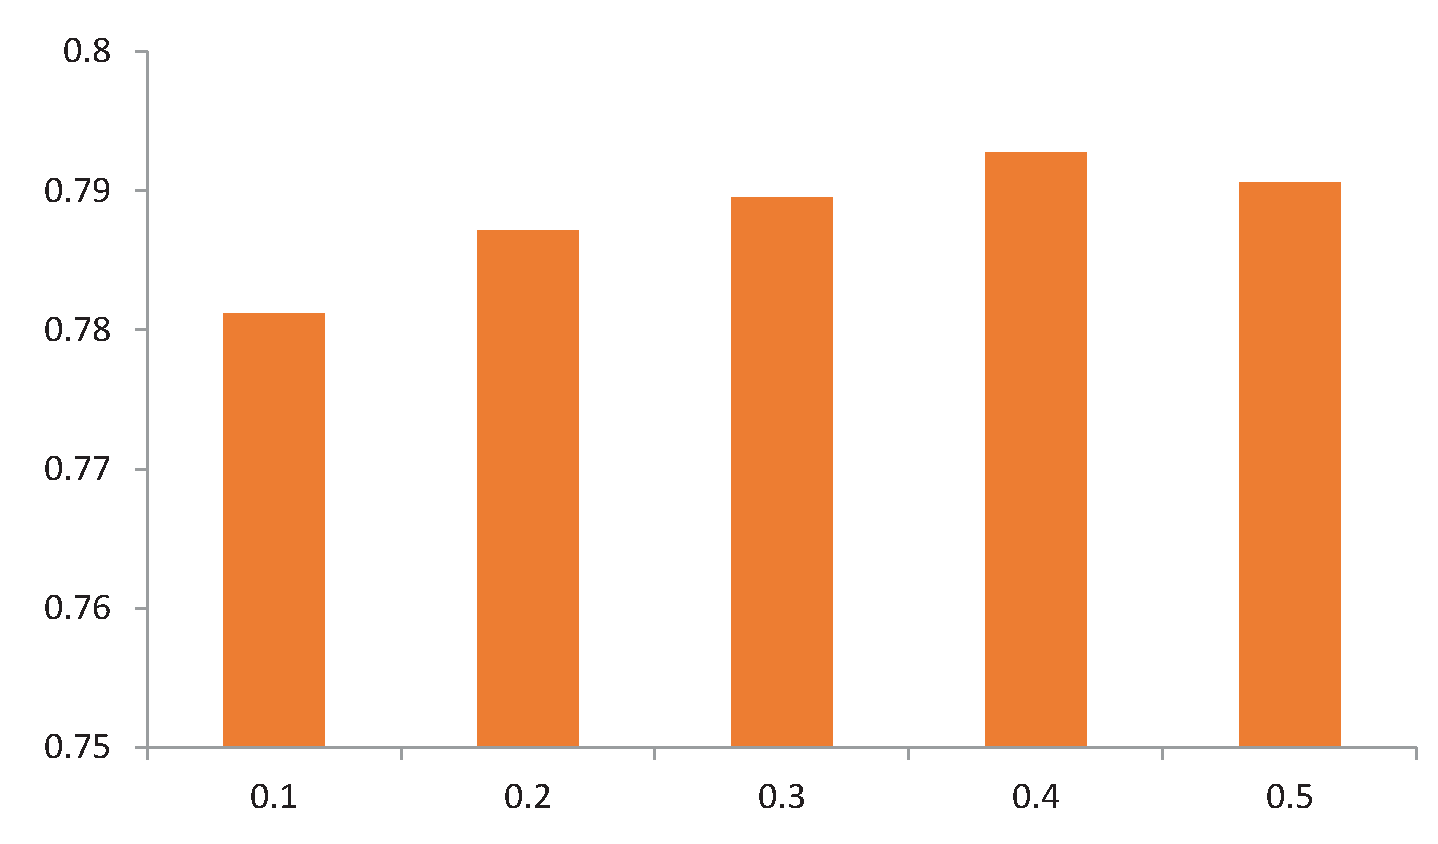
\includegraphics[width=0.5\textwidth]{lambdaPA.eps}
\label{fig:lambdaPA}
}
\caption{Parameter tuning for \textbf{PA} strategy}
\end{figure}

\begin{figure}
\subfigure[NDCG$@$10 for various $\mu$, with $\epsilon=1$]{
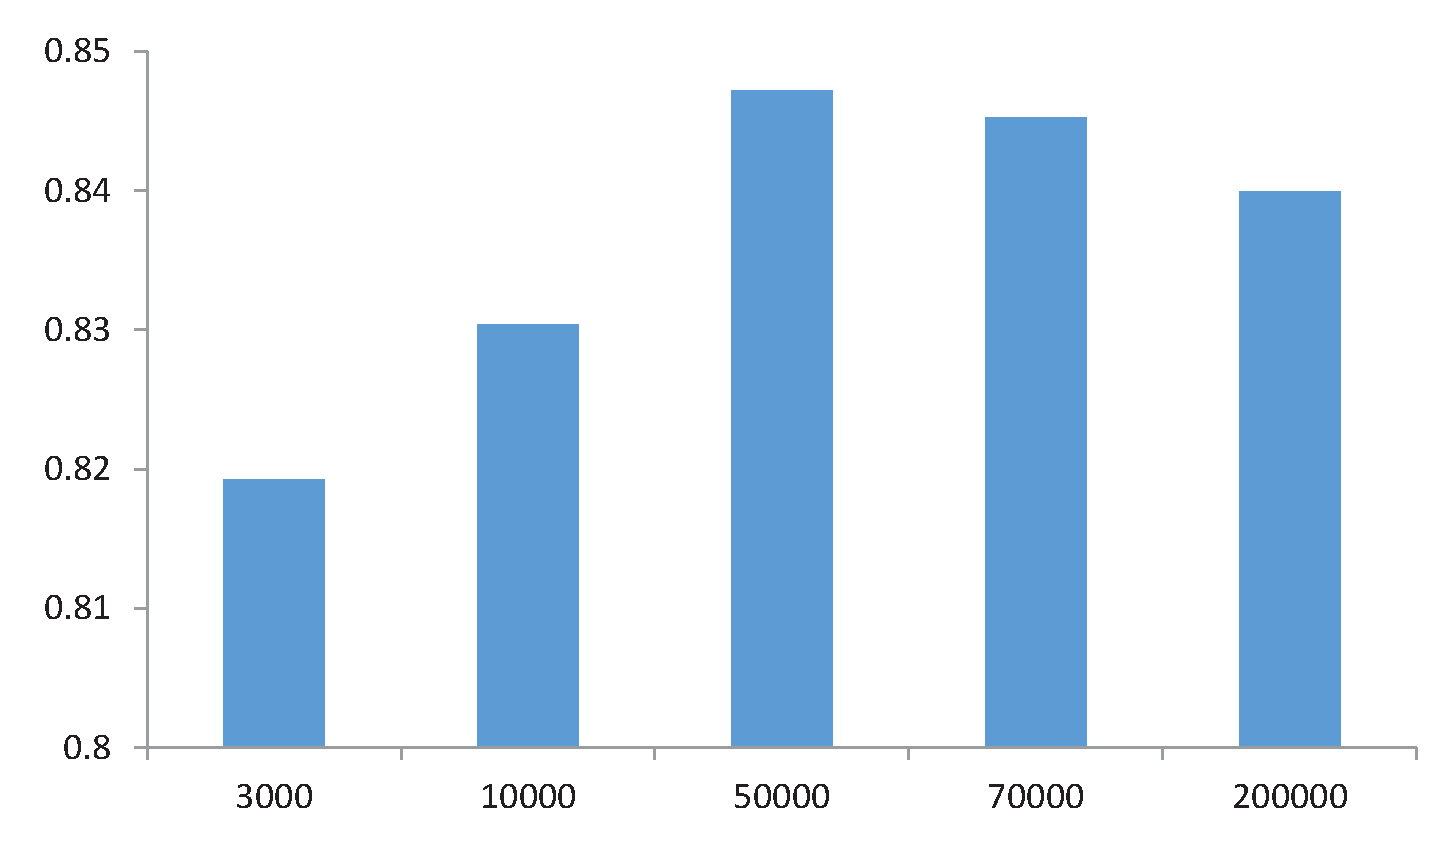
\includegraphics[width=0.5\textwidth]{muPC.eps}
\label{fig:muPC}
}
\subfigure[NDCG$@$10 for various $\epsilon$, with $\mu=10000$]{
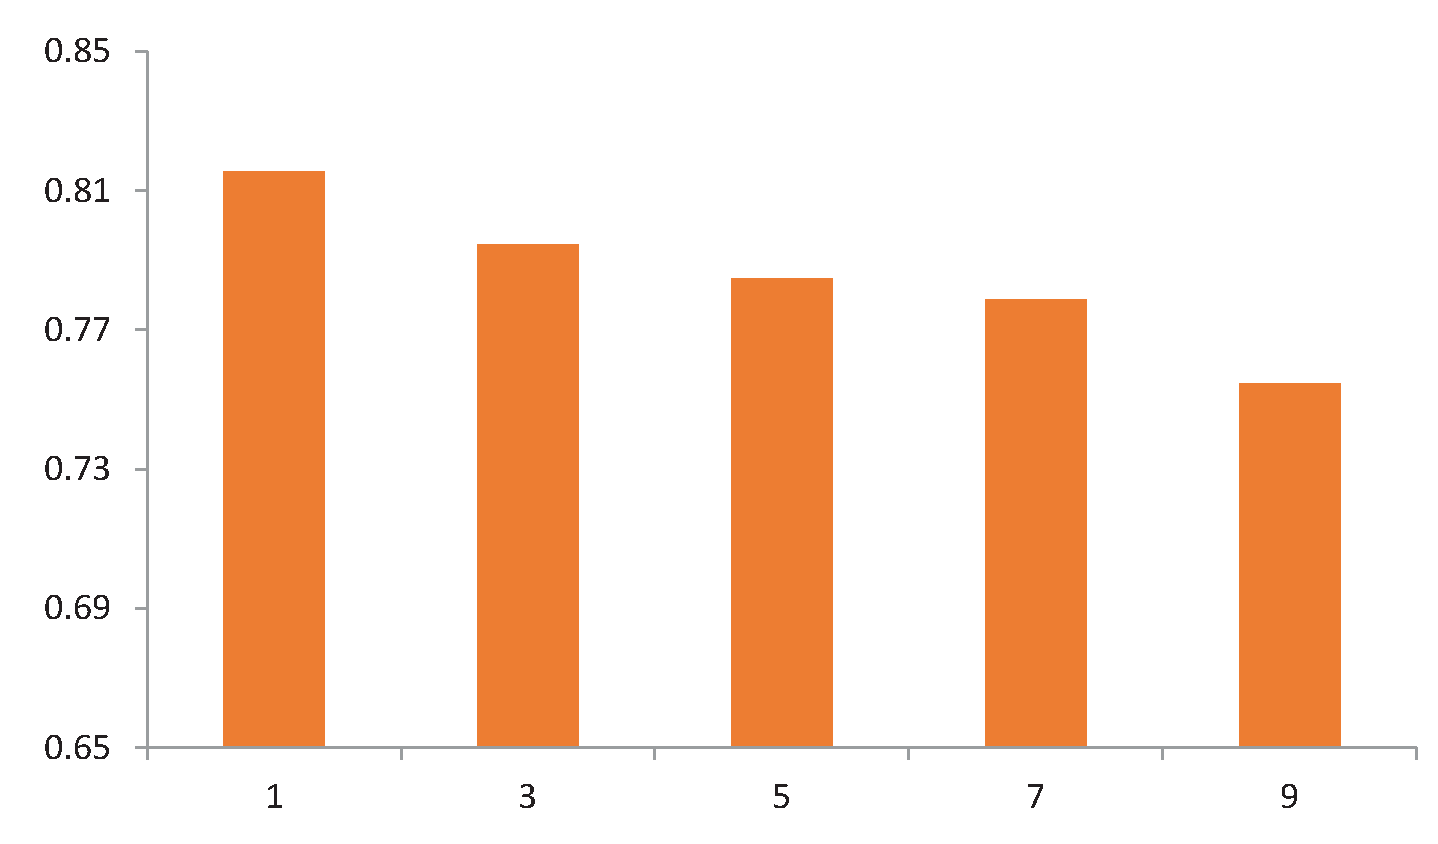
\includegraphics[width=0.5\textwidth]{epsilonPC.eps}
\label{fig:epsilonPC}
}
\caption{Parameter tuning for \textbf{PC} strategy}
\end{figure}

\subsection{Proximity Aggregation Strategy}
We next study the performance of four aggregation strategies. The comparison is carried in the hotel dataset, Beijing category. Parameters $\mu=80000,\sigma+200/3$ for \textbf{PP},$\mu=1000,\lambda=0.2$ for \textbf{PA}. As shown in Fig.~\ref{fig:aggregation}, \textbf{Min} and \textbf{ClusterMin} both achieve satisfying results. However, the best performance is relevant to the combination of conditional probability and aggregation strategies. For \textbf{PA}, the conditional probability is a linear combination of the confidential probability and the global statistics, thus the aggregation strategy has a smaller impact. Surprisingly, \textbf{Ave} is worse than \textbf{Max}. The underlying reason for this unexpected phenomena might be that, under the \textbf{Ave} aggregation, relevant products which receive many reviews will be dragged down by negative reviews, and irrelevant products which receive few reviews will be pushed up consequently. This observation sheds insights to the design of aggregation strategies for general entity search problems.   

\begin{figure}\label{fig:aggregation}
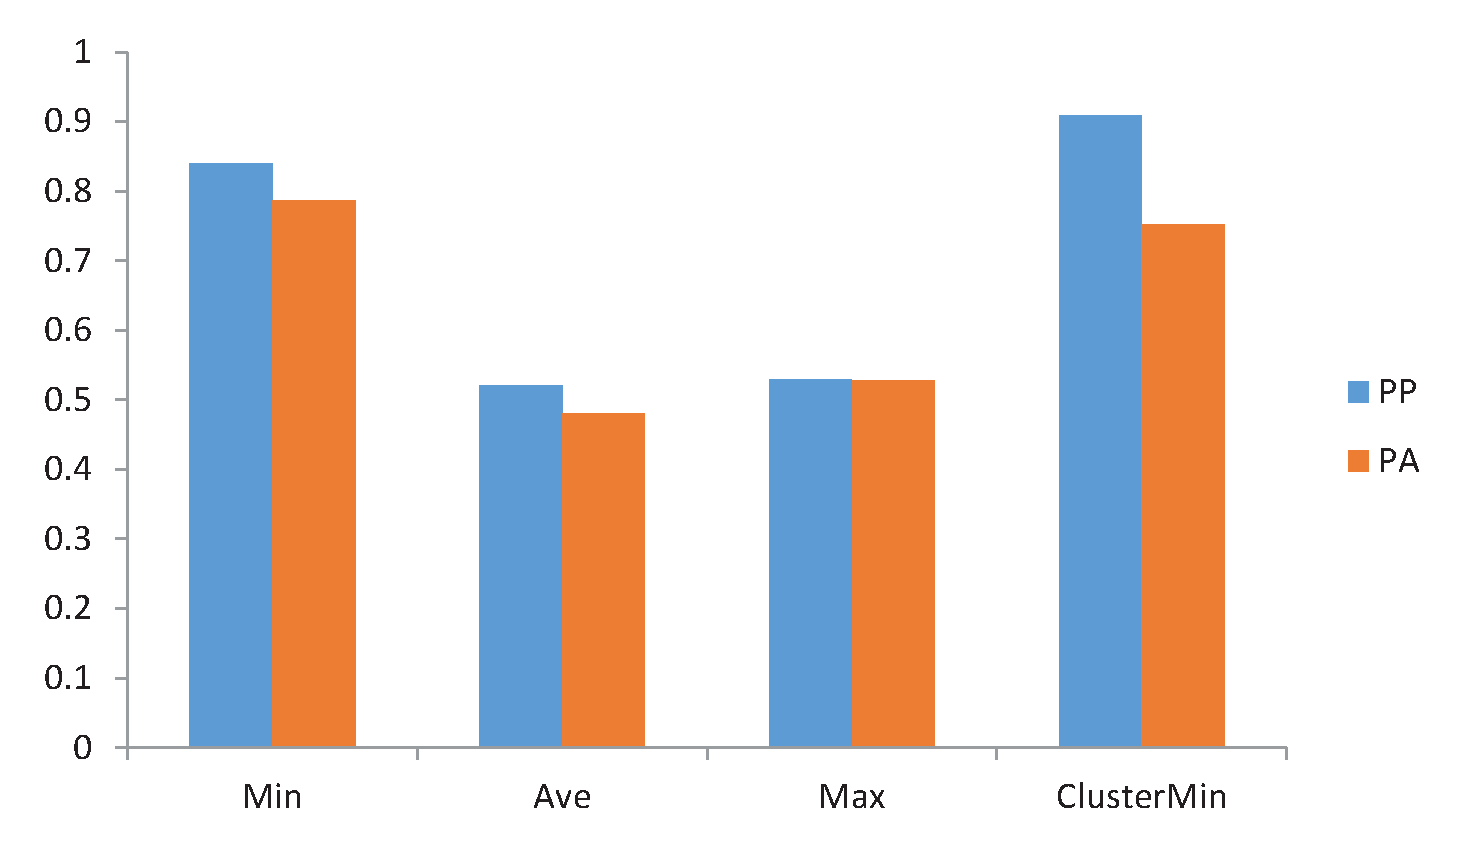
\includegraphics[width=0.5\textwidth]{aggregation.eps}
\caption{NDCG@10 for various aggregations in different conditional prabability paradigm}
\end{figure}

\subsection{Comparative Study}
We finally analyze the performances of our work, compared with state-of-the-art systems. The comparative works include: (1)traditional language modeling framework such as BM25 and PL2~\cite{Ounis2006Terrier}; (2)positional language models such as CRTER~\cite{Zhao2014Modeling},PBM25~\cite{He2011Modeling}, MRF~\cite{Metzler2005Markov} and PLM~\cite{Lv2009Positional}. The positional language models are not dedicated to entity search scenarios, for that reason, we first rank the reviews, and then re-rank the products by counting the number of reviews for each product in the top 100 search results; (3)product search framework, i.e. OpinionRank~\cite{Ganesan2012Opinion} without query expansion. Parameters $\mu=80000,\sigma+200/3$ for \textbf{PP},$\mu=1000,\lambda=0.4$ for \textbf{PA}, $\mu=50000,\epsilon=1$ for \textbf{PA}. For computational efficiency, we use \textbf{Min} aggregation for all strategies. From Tab.~\ref{tab:comparative}, we have the following conclusions. (1) In general, positional language models outperform traditional language models, which highlight the importance of proximity constraints in product search problems. (2) Algorithms that are designed for product search perform significantly better than the re-ranking scheme based on document retrieval. A unified model is neccessary to ensemble document evidences for an entity. (3) Our models are comparable to OpinionRank. Among the three paradigms, \textbf{PP} is most stable and generally obtains best results, which verifies the competency of our contribution.
\begin{table}
\tiny
\begin{tabular}{|c|c|c|c|c|c|c|c|c|c|c|}
\hline
models &	BM25	&PL2	&rrCRTER	&rrPBM25	&rrMRF	&PLM	&OpinionRank	&PP	&PA	&PC\\\hline
\multicolumn{11}{|c|}{hotels}\\\hline										
beijing &	0.5179 &	0.5234	& 0.7620	& 0.7753	& 0.7685	& 0.8276	& \textbf{0.8521} &	0.8346 &	0.7927 &	0.8472 \\\hline
dubai	& 0.6160	& 0.6228	& 0.7066& 	0.6450	& 0.6400	& 0.8106	& 0.8401& 	\textbf{0.8579}& 	0.7149& 	0.8246\\\hline
new-delhi& 	0.4323& 	0.4360& 	0.6532& 	0.6319& 	0.6576& 	0.7462& 	\textbf{0.8130}& 	0.8045& 	0.6820	& 0.7345\\\hline
san-francisco& 	0.4551	& 0.4619& 	0.6532& 	0.7839	& 0.7603	& 0.8227& 	0.8130	& \textbf{0.8702}	& 0.8328	& 0.8274\\\hline
shanghai& 	0.5097& 	0.5206& 	0.6865& 	0.7249	& 0.7603	& 0.8178& 	0.8239& 	\textbf{0.8276}& 	0.7460& 	0.7849\\\hline
Average & 0.5062	&0.5129	&0.6923	&0.7122&	0.7173&	0.8050&	0.8284	&\textbf{0.8389}&	0.7537&	0.8037 \\\hline
\multicolumn{11}{|c|}{cars}\\\hline											
2007	&0.8908&	0.8900&	0.9259	&0.9133&	0.9152	&0.9349&	\textbf{0.9458}&	0.9443	&0.9369	&0.9198\\\hline
2008&	0.8781&	0.8788&	0.9167&	0.9174&	0.9257	&0.9308&	0.9347&	\textbf{0.9376}	&0.9248&	0.9179\\\hline
2009	&0.9176&	0.9163	&0.9256&	0.9129&	0.9257&	0.9186&	0.9494	&\textbf{0.9526}&	0.9430&	0.9320\\\hline
Average &	0.8955&	0.8950	&0.9227	&0.9145&	0.9222&	0.9281&	0.9429	&\textbf{0.9453}&	0.9349&	0.9233\\\hline
\end{tabular}
\caption{Performance of various product search systems}\label{tab:comparative}
\end{table}



\section{Conclusion}
In this paper we present a positional language model for product search problems. Our contributions are two-fold: (1) we incorporate pairwise proximity into the estimation of conditional probability of generating an opinion given a product feature; (2) we explore the aggregation strategies to ensemble review evidences to evaluate the relevance of a product. Experiments on real data sets verify the competence of the presented framework. In the future, we plan to extend the model to tollerate noisy query segmentation. Also, clustering on the fly is a potential direction to speed up the computation for \textbf{ClusterMin} aggregation. 


%\blinddocument
%\bibliographystyle{elsarticle-harv}
\bibliography{C:/scratch/MyPaper/reference}
\end{document}
